%\section{Time}
Time is one of the several methods to verify the location of a node in the positioning systems. There are two different ways for obtain time measurement, which includes Time of Arrival (ToA) and Time Difference of Arrival (TDoA). These two techniques are widely used for detemining the position of a node or target.

\subsection{Time of Arrival (ToA)}

Usually an object at an unknown location is able to create signals at an unknown initial time. This signal can be detected by a set of sensor devices. Every sensor makes an estimation of the Time of Arrival of a signal. So, this method is based on the fact that when exactly the target sends a signal, the exact time the signal will be received by the sensor device and also the velocity of the signal \cite{brian17}.

\begin{figure}[htp]
    \centering
    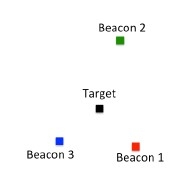
\includegraphics[width=3cm]{1.jpg}
    \caption{the location of Target and Beacons \cite{brian17}}
    \label{fig:Target location}
\end{figure}

In the following example, we have a target which surrounded by some Beacons. At time $t_1$ Beacon one sends a signal to the target, which the Target receives the signal at time $t_2$. Now the distance has to be calculated between the Target and Beacon one($d_1$). According to Fig. 2, the next step is to draw a circle of possible location. The other two Beacons will send a signal to the target and then calculate the distance as the Beacon 1.

\begin{figure}[htp]
    \centering
    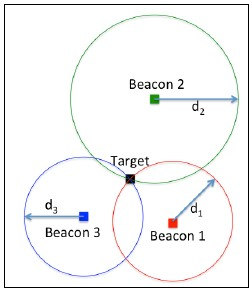
\includegraphics[width=2cm]{2.jpg}
    \caption{Localization \cite{jin18}}
    \label{fig:Localization}
\end{figure}

As mentioned before, the exact time of sending and receiving of a signal and the speed of signal (speed of light is considered) are requirements for calculating the distance.\cite{brian17}

Let the $t_s$ be the time which the emitter sends the signal and $t_a$ is the time which arrives to the target or target receives the signal. c is the speed of light.

Using this formula d (the distance) can be calculated and is used to determine the location of the target. ToA technique requires highly accurate synchronization of sender and receiver clocks \cite{jin18}



\begin{figure}[htp]
	\centering
	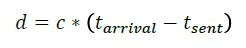
\includegraphics[width=4cm]{3.jpg}
	\caption{distance formula \cite{jin18}}
	\label{fig:Localization}
\end{figure}



\subsection{Time Difference of Arrival (TDoA)}
Time Difference of Arrival technique which is also called multilateration which is often used in radar systems for localization of mobile targets \cite{schaefer15}. In this technique, three or more receivers at different locations capture the signal. The next step is the evaluation of the difference in arrival time of the signal. Because of the varying distances between transmitter and receivers, the signal arrives at different times for different receivers. The difference in arrival time is called TDoA \cite{brian17}.
For example, consider two Beacons (receivers) that received the signal at different points. Using this equation, we want to calculate the distance:

\begin{figure}[htp]
    \centering
    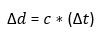
\includegraphics[width=3cm]{4.jpg}
    \caption{distance formula \cite{jin18}}
    \label{fig:formula}
\end{figure}

Say c is the speed of light and Delta t is the difference in arrival times at different Beacons \cite{schaefer18}. Above mentioned equation is applicable to the two dimensions where $(x_1,y_1)$ and $(x_2,y_2)$ would be the positions of Beacons.



\begin{figure}[htp]
    \centering
    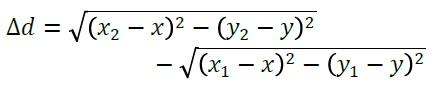
\includegraphics[width=6cm]{5.jpg}
    \caption{distance formula for two dimension \cite{schaefer1}}
    \label{fig:formula}
\end{figure}




Consider $v_1$ and $v_2$ as synchronized versifiers (beacons in above example). The time of received signal is calculated using this equation:

\begin{figure}[htp]
    \centering
    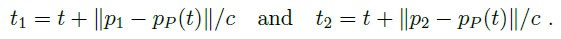
\includegraphics[width=8cm]{6.jpg}
    \caption{Time of received signal \cite{schaefer18}}
    \label{fig:formula}
\end{figure}


The Time Difference of Arrival will be calculated after collecting all the timestamps. Using this formula we wil have TDoA:


\begin{figure}[htp]
    \centering
    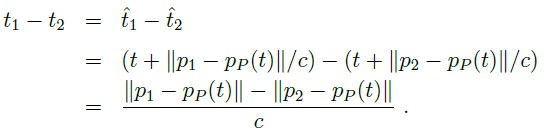
\includegraphics[width=8cm]{7.jpg}
    \caption{Calculating Time Difference of Arrival \cite{schaefer18}}
    \label{fig:formula}
\end{figure}

In this equation only $p_p(t)$ has not given and it indicates the position of the Target! As you can see in the Fig. 3 the intersection of the different hyperbolas is the location of the $p_p(t)$ or the Target. \cite{brian17}

\begin{figure}[htp]
    \centering
    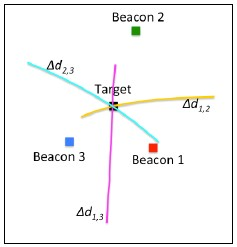
\includegraphics[width=4cm]{8.jpg}
    \caption{possible location in relation to all Beacons \cite{brian17}}
    \label{fig:fig}
\end{figure}

The more versifier (Beacon) we have, one extra hyperbola will be added which will also cross the $p_p(t)$ \cite{schaefer18}.

\subsection{Pro}
ToA technique does not need several information to estimate the location, this becomes one of the advantages of the ToA. The main advantage of the TDoA is that it does not require the communication between the emitter and the receiver. As there no communication in between, there would be no attacking to the system in order to identify the position of the Target. From a security prospective, this is a good point of the TDoA \cite{schaefer18}. Comparing to ToA, Time Difference of Arrival technique is quite beneficial due to requiring less computational power and also inexpensive and simple equipments.


\subsection{Cons}
The major disadvantage for the TDoA is the fact that it needs several measurements to calculate the location. In contrast, ToA does not require a lot of data to calculate the location. As a result, ToA technique need to synchronize the base station and mobile station in order to achieve the estimation of location without need for several information. One of the main weakness of TDoA systems is that it needs very accurate time synchronization which as a result, it makes this technique very expensive to adopt \cite{gante13}.

\subsection{Security Analysis}
Several protocols and approaches have been developed for detecting attacks on ToA and TDoA. However, before examining this approaches we have to know which kind of attack models could be occurred in such systems. Srdjan et al \cite{srivastava}have observed two kind of attacks: internal and external. Internal attacks are which an attacker can report a false position of a node. External attacks are able to convince both node and localization system that the node is not in its true position. These attacks could occur by reporting
false signal strengths and times of signal sending or receiving.

For example, consider Time Difference of Arrival systems which an attacker could be able to send signals to base stations at different times. This type of attack is in the category of Internal Attacks. Jamming is the type of attack that can occur in the system and is a type of External Attack. with jamming, the attacker can run timing attack that is possible with delaying the signal. An internal attack in the localization system could be also false position report. According to Srdjan et al's protocol, it is able to detect false position reports with checking the distance and also the regularity of the reported position \cite{srivastava}.

The most important privacy concern in TDoA Network is that, nodes reveal their location to any station that requests for a location verification. As a result, an attacker is able to send a location verification request to a node and know where exactly it is located \cite{srivastava}. As Srdjan et al stated, by using authentication is it possible to prevent such threats.